\documentclass[11pt]{article}

\usepackage[margin=1in]{geometry}
\usepackage[T1]{fontenc}
\usepackage[utf8]{inputenc}
\usepackage{lmodern}
\usepackage{microtype}
\usepackage{xcolor}
\usepackage{amsmath,amssymb,amsthm,mathtools}
\usepackage{bm}
\usepackage{array,booktabs,longtable,multirow}
\usepackage{enumitem}
\usepackage{tikz}
\usepackage{hyperref}
\usepackage[most]{tcolorbox}
\usepackage{fancyhdr}
\usepackage{titlesec}
\usepackage{graphicx}

\hypersetup{
  colorlinks=true,
  linkcolor=blue!50!black,
  urlcolor=blue!50!black,
  citecolor=blue!50!black,
  pdftitle={Coding Theory Lecture Notes: Linear Codes},
  pdfauthor={OpenAI}
}

\definecolor{accent}{HTML}{1F4E79}
\definecolor{softaccent}{HTML}{EAF2F8}
\definecolor{softgray}{HTML}{F6F7F9}

\titleformat{\section}{\Large\bfseries\color{accent}}{\thesection.}{0.6em}{}
\titleformat{\subsection}{\large\bfseries\color{accent}}{\thesubsection}{0.6em}{}
\titleformat{\subsubsection}{\normalsize\bfseries\color{accent}}{\thesubsubsection}{0.6em}{}

\setlist[itemize]{topsep=4pt,itemsep=3pt}
\setlist[enumerate]{topsep=4pt,itemsep=3pt}
\renewcommand{\arraystretch}{1.25}
\setlength{\parskip}{0.55em}
\setlength{\parindent}{0pt}

\pagestyle{fancy}
\fancyhf{}
\lhead{\textcolor{accent}{Coding Theory: Linear Codes}}
\rhead{\textcolor{accent}{\thepage}}
\renewcommand{\headrulewidth}{0.4pt}
\renewcommand{\headrule}{\hbox to\headwidth{\color{accent}\leaders\hrule height \headrulewidth\hfill}}

\newtheorem{definition}{Definition}[section]
\newtheorem{proposition}[definition]{Proposition}
\newtheorem{theorem}[definition]{Theorem}
\newtheorem{lemma}[definition]{Lemma}
\newtheorem{corollary}[definition]{Corollary}
\newtheorem{example}[definition]{Example}
\newtheorem{exercise}[definition]{Exercise}

\newtcolorbox{keyidea}{
  colback=softaccent,
  colframe=accent,
  boxrule=0.6pt,
  arc=2mm,
  left=2mm,right=2mm,top=1.5mm,bottom=1.5mm,
  title=Key idea,
  fonttitle=\bfseries
}

\newtcolorbox{summarybox}{
  colback=softgray,
  colframe=black!20,
  boxrule=0.4pt,
  arc=2mm,
  left=2mm,right=2mm,top=1.5mm,bottom=1.5mm
}

\newenvironment{solution}{\begin{tcolorbox}[colback=white,colframe=accent!45,title=Solution,boxrule=0.5pt,arc=1.5mm]}{\end{tcolorbox}}

\newcommand{\F}{\mathbb{F}}
\newcommand{\code}{\mathcal{C}}
\newcommand{\vect}[1]{\bm{#1}}
\newcommand{\transpose}{^{\mathsf T}}

\begin{document}

\begin{titlepage}
  \centering
  \vspace*{2cm}
  {\Huge\bfseries\color{accent} Coding Theory: Linear Codes\par}
  \vspace{0.5cm}
  {\Large Lecture Notes in LaTeX\par}
  \vspace{1.2cm}
  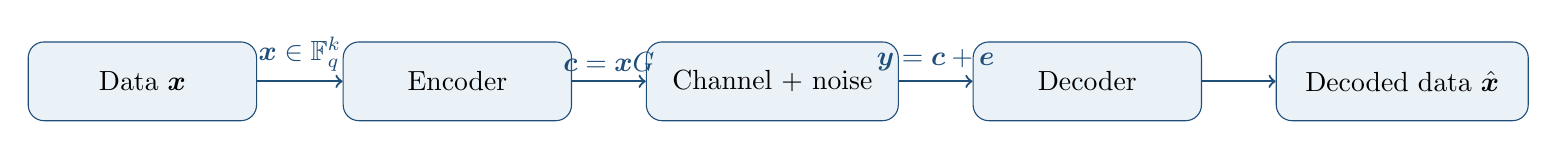
\begin{tikzpicture}[scale=1]
    \node[draw=accent,rounded corners=2mm,fill=softaccent,minimum width=2.9cm,minimum height=1cm] (tx) at (0,0) {Data $\vect{x}$};
    \node[draw=accent,rounded corners=2mm,fill=softaccent,minimum width=2.9cm,minimum height=1cm] (enc) at (4,0) {Encoder};
    \node[draw=accent,rounded corners=2mm,fill=softaccent,minimum width=3.2cm,minimum height=1cm] (chan) at (8,0) {Channel + noise};
    \node[draw=accent,rounded corners=2mm,fill=softaccent,minimum width=2.9cm,minimum height=1cm] (dec) at (12,0) {Decoder};
    \node[draw=accent,rounded corners=2mm,fill=softaccent,minimum width=3.2cm,minimum height=1cm] (rx) at (16,0) {Decoded data $\hat{\vect{x}}$};
    \draw[->,thick,accent] (tx) -- node[above] {$\vect{x}\in\F_q^k$} (enc);
    \draw[->,thick,accent] (enc) -- node[above] {$\vect{c}=\vect{x}G$} (chan);
    \draw[->,thick,accent] (chan) -- node[above] {$\vect{y}=\vect{c}+\vect{e}$} (dec);
    \draw[->,thick,accent] (dec) -- (rx);
  \end{tikzpicture}
  \vfill
  \begin{summarybox}
  \textbf{Scope of these notes.} These notes reorganize the ``Linear Codes'' slide deck into a continuous lecture-note format. They cover finite fields, linear encodings, \((n,k)\) linear codes, generator matrices, systematic form, repetition and parity-check codes, and parity-check matrices.
  \end{summarybox}
  \vfill
  {\large \today\par}
\end{titlepage}

\tableofcontents
\newpage

\section{What is coding theory?}

Coding theory studies how to transmit or store information reliably in the presence of corruption. In a communication setting, a sender starts with information symbols, transforms them into an encoded word, sends that word through a noisy channel, and the receiver tries to recover the original data from the corrupted output.

\begin{keyidea}
The central principle is redundancy: we intentionally add structured extra symbols so that the receiver can detect or correct corruption.
\end{keyidea}

A generic communication model has the form
\[
\vect{x}=(x_1,\dots,x_k)
\xrightarrow{\text{encoder}}
\vect{c}=(c_1,\dots,c_n)
\xrightarrow{\text{noise }\vect e}
\vect{y}=\vect{c}+\vect{e}
\xrightarrow{\text{decoder}}
\hat{\vect{x}}=(\hat x_1,\dots,\hat x_k),
\]
where usually \(n\ge k\). The vector \(\vect{c}\) is called a \emph{codeword}.

\subsection{Encoding}

Let \(A\) be an alphabet. An \emph{encoding} is a map
\[
A^k \longrightarrow A^n,
\qquad
(x_1,\dots,x_k)\longmapsto (c_1,\dots,c_n),
\]
with \(n\ge k\). The output vector \(\vect c=(c_1,\dots,c_n)\) is the transmitted codeword.

\begin{example}[A first encoding]
When \(k=1\), a very simple encoding repeats the same symbol:
\[
(x_1)\longmapsto (x_1,x_1,\dots,x_1)\in A^n.
\]
If the alphabet is binary, \(A=\{0,1\}\), then
\[
(0)\mapsto (0,0,\dots,0),
\qquad
(1)\mapsto (1,1,\dots,1).
\]
This is called the \emph{repetition code}.
\end{example}

\section{Discrete alphabets and finite fields}

In linear coding theory, alphabets are usually finite fields. The first examples come from arithmetic modulo a prime.

\subsection{Arithmetic modulo \texorpdfstring{$p$}{p}}

For a prime number \(p\), arithmetic modulo \(p\) means that every computation is reduced by taking its remainder upon division by \(p\). The resulting set is
\[
\F_p=\{0,1,\dots,p-1\}.
\]

\subsubsection*{Addition and multiplication modulo \texorpdfstring{$2$}{2}}

\[
\begin{array}{c|cc}
+ & 0 & 1 \\\hline
0 & 0 & 1 \\
1 & 1 & 0
\end{array}
\qquad
\begin{array}{c|cc}
\cdot & 0 & 1 \\\hline
0 & 0 & 0 \\
1 & 0 & 1
\end{array}
\]

\subsubsection*{Addition and multiplication modulo \texorpdfstring{$3$}{3}}

\[
\begin{array}{c|ccc}
+ & 0 & 1 & 2 \\\hline
0 & 0 & 1 & 2 \\
1 & 1 & 2 & 0 \\
2 & 2 & 0 & 1
\end{array}
\qquad
\begin{array}{c|ccc}
\cdot & 0 & 1 & 2 \\\hline
0 & 0 & 0 & 0 \\
1 & 0 & 1 & 2 \\
2 & 0 & 2 & 1
\end{array}
\]

\subsection{What goes wrong modulo a composite number?}

If we work modulo a non-prime integer, arithmetic no longer behaves like field arithmetic.

For example, modulo \(4\):
\[
2\cdot 2\equiv 0\pmod 4.
\]
This has several consequences:
\begin{itemize}
  \item from \(2x=0\), we cannot conclude \(x=0\), because \(x=2\) also works;
  \item a degree-1 equation may have more than one solution;
  \item two nonzero numbers can multiply to zero, so \emph{zero divisors} appear;
  \item equations such as \(2x=1\) can have no solution at all.
\end{itemize}

\begin{exercise}
Prove that if \(m\) is not prime, then integers modulo \(m\) do not form a field.
\end{exercise}

\begin{solution}
If \(m\) is composite, then \(m=ab\) for some integers \(a,b\) with \(1<a<m\) and \(1<b<m\). Modulo \(m\), we have
\[
ab\equiv 0\pmod m.
\]
Hence the class of \(a\) is nonzero and the class of \(b\) is nonzero, but their product is zero. In a field, this cannot happen: nonzero elements must be invertible, and a product of two nonzero elements cannot be zero. Therefore \(\mathbb Z/m\mathbb Z\) is not a field when \(m\) is composite.
\end{solution}

\subsection{The finite field \texorpdfstring{$\F_p$}{Fp}}

\begin{definition}
For a prime \(p\), the set of integers modulo \(p\), denoted \(\F_p\), is a \emph{finite field}. This means:
\begin{itemize}
  \item it has exactly \(p\) elements;
  \item addition, subtraction, and multiplication are defined and satisfy the usual commutative laws;
  \item every nonzero element has a multiplicative inverse.
\end{itemize}
\end{definition}

\begin{example}[Inverse modulo \texorpdfstring{$5$}{5}]
In \(\F_5\), the inverse of \(3\) is \(2\) because
\[
3\cdot 2 = 6 \equiv 1 \pmod 5.
\]
\end{example}

\begin{example}[Elements that are their own inverse modulo \texorpdfstring{$7$}{7}]
In \(\F_7\), the elements \(1\) and \(6\) are self-inverse because
\[
1\cdot 1\equiv 1\pmod 7,
\qquad
6\cdot 6 = 36 \equiv 1\pmod 7.
\]
\end{example}

\subsection{Another finite field: \texorpdfstring{$\F_4$}{F4}}

Finite fields do not only exist when the number of elements is prime. There is also a field with four elements. One way to describe it is to introduce an element \(\omega\) satisfying
\[
\omega^2+\omega+1=0 \quad \text{over }\F_2.
\]
Equivalently,
\[
\omega^2=\omega+1,
\qquad
\omega^3=1.
\]
Then
\[
\F_4=\{0,1,\omega,\omega^2\}.
\]

Its addition and multiplication tables are:
\[
\begin{array}{c|cccc}
+ & 0 & 1 & \omega & \omega^2 \\\hline
0 & 0 & 1 & \omega & \omega^2 \\
1 & 1 & 0 & \omega^2 & \omega \\
\omega & \omega & \omega^2 & 0 & 1 \\
\omega^2 & \omega^2 & \omega & 1 & 0
\end{array}
\qquad
\begin{array}{c|cccc}
\cdot & 0 & 1 & \omega & \omega^2 \\\hline
0 & 0 & 0 & 0 & 0 \\
1 & 0 & 1 & \omega & \omega^2 \\
\omega & 0 & \omega & \omega^2 & 1 \\
\omega^2 & 0 & \omega^2 & 1 & \omega
\end{array}
\]

\begin{summarybox}
From now on we write \(\F_q\) for a finite field with \(q\) elements. Typical examples are \(\F_p\) for prime \(p\), and also extension fields such as \(\F_4\).
\end{summarybox}

\section{Linear encoding and linear codes}

Once the alphabet is a finite field \(\F_q\), the ambient space \(\F_q^n\) becomes a vector space. This allows us to use linear algebra to design codes.

\subsection{Linear encoding}

\begin{definition}
A \emph{linear encoding} over \(\F_q\) is a linear map
\[
\F_q^k \longrightarrow \F_q^n,
\qquad
\vect{x}\longmapsto \vect{c}.
\]
\end{definition}

Because the map is linear:
\begin{itemize}
  \item the sum of two codewords is again a codeword;
  \item any scalar multiple of a codeword is again a codeword.
\end{itemize}

\begin{definition}
A subset \(\code\subseteq \F_q^n\) is called a \emph{linear code} if it is a linear subspace of \(\F_q^n\).
\end{definition}

If \(\code\) is a linear subspace of dimension \(k\), then \(\code\) is called an \((n,k)\) linear code over \(\F_q\). The integer \(n\) is the \emph{length}, and \(k\) is the \emph{dimension}.

\subsection{Basic properties}

If \(\code\) is a linear code, then automatically:
\begin{itemize}
  \item the zero codeword \(\vect 0\) belongs to \(\code\);
  \item whenever \(\vect c\in \code\), also \(-\vect c\in \code\);
  \item every codeword is a linear combination of basis vectors of \(\code\).
\end{itemize}

\begin{proposition}
If \(\code\) is an \((n,k)\) linear code over \(\F_q\), then
\[
|\code|=q^k.
\]
\end{proposition}

\begin{proof}
Choose a basis \(\vect b_1,\dots,\vect b_k\) of \(\code\). Every codeword can be written uniquely as
\[
x_1\vect b_1+\cdots+x_k\vect b_k,
\qquad x_i\in \F_q.
\]
Each coefficient \(x_i\) has \(q\) choices, and there are \(k\) independent coefficients. Therefore the number of codewords is \(q^k\).
\end{proof}

\section{Generator matrices}

Linear maps between finite-dimensional vector spaces are represented by matrices. In coding theory, the matrix representing the encoding map is called a generator matrix.

\begin{definition}
Let \(\code\) be an \((n,k)\) linear code over \(\F_q\). A \emph{generator matrix} for \(\code\) is a \(k\times n\) matrix \(G\) whose rows form a basis of \(\code\).
\end{definition}

If \(\vect{x}=(x_1,\dots,x_k)\in \F_q^k\), then encoding is given by
\[
\vect{c}=\vect{x}G.
\]

\subsection{Systematic form}

A particularly convenient generator matrix has the form
\[
G=[I_k\mid A],
\]
where \(I_k\) is the \(k\times k\) identity matrix and \(A\) is a \(k\times (n-k)\) matrix.

\begin{definition}
A code is said to be in \emph{systematic form} if it has a generator matrix of the form \(G=[I_k\mid A]\).
\end{definition}

In this case, the first \(k\) coordinates of the codeword are exactly the information symbols. If
\[
\vect{x}=(x_1,\dots,x_k),
\]
then
\[
\vect{x}G=(x_1,\dots,x_k,c_{k+1},\dots,c_n).
\]
So the information symbols appear explicitly in the transmitted codeword, followed by the parity symbols.

\subsection{Example: repetition code}

The \((n,1)\) repetition code sends
\[
(x_1)\longmapsto (x_1,x_1,\dots,x_1).
\]
Its generator matrix is simply
\[
G=[1\;1\;\cdots\;1].
\]
Indeed,
\[
(x_1)G=(x_1,x_1,\dots,x_1).
\]

\subsection{Example: single parity-check code}

The \((n,n-1)\) single parity-check code is defined by
\[
(x_1,\dots,x_k)\longmapsto (x_1,\dots,x_k, x_1+\cdots+x_k),
\]
where \(k=n-1\).

A generator matrix in systematic form is
\[
G=
\begin{bmatrix}
1 & 0 & \cdots & 0 & 1 \\
0 & 1 & \cdots & 0 & 1 \\
\vdots & \vdots & \ddots & \vdots & \vdots \\
0 & 0 & \cdots & 1 & 1
\end{bmatrix}
=[I_k\mid \vect{1}],
\]
where the last column consists entirely of ones.

Multiplying gives
\[
(x_1,\dots,x_k)G=(x_1,\dots,x_k,x_1+\cdots+x_k).
\]

\begin{keyidea}
In systematic form, the generator matrix shows exactly how redundancy is added to the original data.
\end{keyidea}

\section{Worked exercises on linearity}

\subsection{A codebook that is not linear}

\begin{exercise}
Consider the codebook of length \(4\) over \(\F_2\):
\[
\{(1,0,0,0),\ (0,1,0,1),\ (1,1,0,1),\ (0,0,0,1)\}.
\]
Is this a linear code? If so, provide a generator matrix.
\end{exercise}

\begin{solution}
This codebook is \emph{not} linear.

First, a linear code must contain the zero vector \((0,0,0,0)\), but this vector is not in the codebook.

Second, linear codes must be closed under addition. In \(\F_2\),
\[
(1,1,0,1)+(0,0,0,1)=(1,1,0,0),
\]
and this vector also does not belong to the codebook. Therefore the set is not a linear code.
\end{solution}

\subsection{A codebook that is linear}

\begin{exercise}
Consider the following codebook of length \(5\) over \(\F_2\):
\begin{align*}
&(0,0,0,0,0),\ (1,0,0,1,0),\ (0,1,0,1,1),\ (1,1,0,0,1),\\
&(0,0,1,0,1),\ (1,0,1,1,1),\ (0,1,1,1,0),\ (1,1,1,0,0).
\end{align*}
Is this a linear code? If so, provide a generator matrix.
\end{exercise}

\begin{solution}
Yes, this is a linear code. Notice that the first three coordinates run through all vectors of \(\F_2^3\):
\[
(0,0,0),(1,0,0),(0,1,0),(1,1,0),(0,0,1),(1,0,1),(0,1,1),(1,1,1).
\]
This strongly suggests a systematic generator matrix of the form
\[
G=
\begin{bmatrix}
1&0&0&a_{11}&a_{12}\\
0&1&0&a_{21}&a_{22}\\
0&0&1&a_{31}&a_{32}
\end{bmatrix}.
\]
We read off the last two coordinates from the codewords corresponding to the basis vectors:
\[
(1,0,0)\mapsto (1,0,0,1,0),
\]
so the first row is \((1,0,0,1,0)\);
\[
(0,1,0)\mapsto (0,1,0,1,1),
\]
so the second row is \((0,1,0,1,1)\);
\[
(0,0,1)\mapsto (0,0,1,0,1),
\]
so the third row is \((0,0,1,0,1)\).

Hence a generator matrix is
\[
G=
\begin{bmatrix}
1&0&0&1&0\\
0&1&0&1&1\\
0&0&1&0&1
\end{bmatrix}.
\]
Now every codeword is of the form \(\vect{x}G\) with \(\vect{x}\in\F_2^3\), so the codebook is indeed linear.
\end{solution}

\section{Parity-check matrices}

A linear code can be described either by its generators or by the linear equations that all codewords satisfy.

\begin{definition}
Let \(\code\) be an \((n,k)\) linear code over \(\F_q\). A matrix \(H\) of size \((n-k)\times n\) is called a \emph{parity-check matrix} for \(\code\) if
\[
\code=\{\vect{v}\in \F_q^n : H\vect{v}\transpose=0\}.
\]
\end{definition}

Thus codewords are exactly the vectors satisfying a system of \(n-k\) homogeneous linear equations.

\subsection{Parity-check matrix from a systematic generator matrix}

Suppose
\[
G=[I_k\mid A]
\]
is a generator matrix in systematic form, where \(A\) is a \(k\times (n-k)\) matrix.
Then define
\[
H=[-A\transpose\mid I_{n-k}].
\]

\begin{proposition}
If \(G=[I_k\mid A]\), then \(H=[-A\transpose\mid I_{n-k}]\) is a parity-check matrix for the code generated by \(G\).
\end{proposition}

\begin{proof}
First compute
\[
G\transpose=
\begin{bmatrix}
I_k\\
A\transpose
\end{bmatrix}.
\]
Therefore
\[
HG\transpose = [-A\transpose\mid I_{n-k}]
\begin{bmatrix}
I_k\\
A\transpose
\end{bmatrix}
= -A\transpose + A\transpose = 0.
\]
If \(\vect{c}\in \code\), then \(\vect{c}=\vect{x}G\) for some \(\vect{x}\in \F_q^k\). Taking transposes,
\[
\vect{c}\transpose = G\transpose\vect{x}\transpose.
\]
Hence
\[
H\vect{c}\transpose = HG\transpose\vect{x}\transpose = 0.
\]
So every codeword lies in the kernel of the linear map \(\vect v\mapsto H\vect v\transpose\).

Now \(H\) has rank \(n-k\) because its last \(n-k\) columns form the identity matrix. Therefore its kernel has dimension
\[
n-(n-k)=k.
\]
But \(\code\) is already a \(k\)-dimensional subspace contained in this kernel, so they must be equal:
\[
\code = \ker(H).
\]
Thus \(H\) is a parity-check matrix for \(\code\).
\end{proof}

\subsection{Example: parity-check matrix of the repetition code}

For the \((n,1)\) repetition code, the generator matrix in systematic form is
\[
G=[1\mid 1\;1\;\cdots\;1].
\]
Hence \(A\) is the row vector of all ones, so a parity-check matrix is
\[
H=[-A\transpose\mid I_{n-1}]
=
\begin{bmatrix}
-1 & 1 & 0 & \cdots & 0 \\
-1 & 0 & 1 & \cdots & 0 \\
\vdots & \vdots & \vdots & \ddots & \vdots \\
-1 & 0 & 0 & \cdots & 1
\end{bmatrix}.
\]
Over \(\F_2\), we have \(-1=1\), so this becomes
\[
H=
\begin{bmatrix}
1 & 1 & 0 & \cdots & 0 \\
1 & 0 & 1 & \cdots & 0 \\
\vdots & \vdots & \vdots & \ddots & \vdots \\
1 & 0 & 0 & \cdots & 1
\end{bmatrix}.
\]
These equations force all coordinates to be equal, exactly as expected for the repetition code.

\section{Final summary}

\begin{summarybox}
\textbf{Main ideas from this lecture.}
\begin{itemize}
  \item A code adds structured redundancy so that corrupted data can still be recovered.
  \item For linear coding theory, the alphabet is usually a finite field \(\F_q\).
  \item A linear \((n,k)\) code is a \(k\)-dimensional subspace of \(\F_q^n\).
  \item Such a code contains exactly \(q^k\) codewords.
  \item A generator matrix \(G\) describes encoding by \(\vect c=\vect xG\).
  \item In systematic form, \(G=[I_k\mid A]\), so the data symbols appear directly in the codeword.
  \item A parity-check matrix \(H\) describes the code as the solution space of linear equations:
  \[
  \code=\{\vect v\in \F_q^n:H\vect v\transpose=0\}.
  \]
  \item If \(G=[I_k\mid A]\), then a compatible parity-check matrix is \(H=[-A\transpose\mid I_{n-k}]\).
\end{itemize}
\end{summarybox}

\end{document}
